%!TEX root = main.tex
%
% lattices.tex
%

\chapter{Lattices}

Most of the results can be found in \cite{gratzer78}.

\begin{definition}
Let $P$ be a partially ordered set and $a,b \in P$. The \emph{supremum} of $\{a,b\}$, denoted $\sup\{a,b\}$, is the smallest upper bound of the set $\{a,b\}$. Dually, the \emph{infimum} $\inf \{a,b\}$ is the largest lower bound of the set $\{a,b\}$.
\end{definition}
\begin{example}
Suprema and infima need not exist. Consider for instance the following poset.
\[ \begin{tikzcd}
a \arrow[d, no head] \arrow[dr, no head] & b \arrow[dl, no head, crossing over] \arrow[d, no head] \\
c & d
\end{tikzcd} \]
The subset $\{a,b\}$ has no upper bounds at all, and the subset $\{c,d\}$ has no lower bounds at all. The supremum of $\{c,d\}$ also does not exist; the lower bounds of $\{c,d\}$ are $a$ and $b$, but none of the two is the smallest.
\end{example}
\begin{example}
\[ \begin{tikzcd}
  & 1 \arrow[dr, no head] \arrow[dl, no head] &   \\
a \arrow[d, no head] \arrow[drr, no head] &   & b \arrow[dll, no head, crossing over] \arrow[d, no head] \\
c \arrow[dr, no head] &   & d \arrow[dl, no head] \\
  & 0 &
\end{tikzcd} \]
The upper bounds of $\{c,d\}$ are $a$, $b$ and $1$. Yet none of the three upper bounds is a smallest upper bound. The supremum of $a$ and $b$ is $1$. The infimum of $c$ and $d$ is $0$.
\end{example}
\begin{definition}
Let $P$ be a poset. Then $P$ is called a \emph{lattice} if every pair of points has a supremum and an infimum. The supremum of $a,b \in P$ is denoted by $a \vee b := \sup\{a,b\}$. The infimum is denoted by $a \wedge b := \inf\{a,b\}$. The operation $a \vee b$ is called the \emph{join} and the operation $a \wedge b$ is called the \emph{meet}.
\end{definition}
An easy induction argument shows that if $P$ is a lattice, then every finite subset $H \subseteq P$ also has a supremum and infimum.
Consider the empty set $\emptyset$. If $P$ is an arbitrary poset, then $\sup \emptyset \in P$ if and only if $P$ has a unique largest element, which we will call the \emph{top} of $P$, denoted $1 \in P$. Similarly, $\inf \emptyset \in P$ if and only if $P$ has a unique smallest element, which we will call the \emph{bottom} of $P$, denoted $0 \in P$.

\begin{definition}
Let $L$ be a lattice. Then $L$ is called a \emph{bounded lattice} if it has a top and a bottom element.
\end{definition}
Note that the empty set $\emptyset$ is not a bounded lattice, although it is a lattice.
\begin{example}
Consider the set of all positive numbers $\Z_{>0}$, where we define $n \leq m \iff n \mid m$. It's clear that $n \mid n$, that $n \mid m, m \mid n \implies n = m$ and that $n \mid m \mid k \implies n \mid k$. Hence $\leq$ is a partial order on $\Z_{>0}$. Moreover, $a \wedge b = \gcd(a,b)$ and $a \vee b = \lcm(a,b)$. Hence we have found a lattice. The lattice $\Z_{>0}$ has a bottom element, namely $1$. It does not have a top element. Below is a partial picture of the lattice.
\[ \begin{tikzcd}
  & 18 & & 12 & 8 \\
9 \arrow[ur, no head] &   & 6 \arrow[ul, no head] \arrow[ur, no head] & 15 & 4 \arrow[ul, no head] \arrow[u, no head] & 10 & & \cdots \\
  & 3 \arrow[ul, no head] \arrow[ur, no head] \arrow[urr, no head] &   & 2 \arrow[ul, no head, crossing over] \arrow[ur, no head] \arrow[urr, no head] &   & 5 \arrow[ull, no head, crossing over] \arrow[u, no head] & & \cdots \\
  &   &   & 1 \arrow[ull, no head] \arrow[u, no head] \arrow[urr, no head] &   &   & & 
\end{tikzcd} \]
\end{example}
\begin{proposition}
\label{prop:algebraic identities of a lattice}
Let $L$ be a lattice and $a,b,c \in L$. The following is true.
\begin{enumerate}
	\item $a \wedge a = a$, $a \vee a =a$. (idempotency)
	\item $a \wedge b = b \wedge a$, $a \vee b = b \vee a$. (commutativity)
	\item $a \wedge (b \wedge c) = (a \wedge b) \wedge c$, $a \vee (b \vee c) = (a \vee b) \vee c$. (associativity)
\end{enumerate}
\end{proposition}
\begin{proof}
Suprema and infima provide the necessary properties.
\end{proof}
Judging from Proposition \ref{prop:algebraic identities of a lattice}, we can just as well start with an arbitrary set $L$ together with two binary operations $\wedge : L^2 \to L$ and $\vee : L^2 \to L$ such that they satisfy idempotency, commutativity and associativity. This enriches the set $L$ with an algebraic structure $(L, \wedge, \vee)$. We can then turn $L$ into a partially ordered set by declaring
\[ a \leq b \iff a \wedge b = a, \qquad a \leq b \iff a \vee b = b. \]
\begin{lemma}
The following is true.
\begin{enumerate}
	\item $a \leq b \iff a \wedge b = a$, $a \leq b \iff a \vee b = b$.
	\item $a \wedge (a \vee b) = a$, $a \vee (a \wedge b) = a$. (absorption)
\end{enumerate}
\end{lemma}

\begin{definition}
Let $L,M$ be lattices and let $f : L \to M$ be a map of sets. Then $f$ is called a \emph{meet-morphism} or \emph{$\wedge$-morphism} if $f(a \wedge b) = f(a) \wedge f(b)$ for all $a,b \in L$. The map $f$ is called a \emph{join-morphism} or \emph{$\vee$-morphism} if $f(a \vee b) = f(a) \vee f(b)$ for all $a,b \in L$. The map $f$ is called a \emph{morphism} if it is both a meet-morphism and a join-morphism.
\end{definition}
The collection of all lattices together with their morphisms defines a category $\mathbf{Lat}$.
\begin{definition}
Let $L,M$ be bounded lattices and let $f : L \to M$ be a map. Then $f$ is called a \emph{morphism of bounded lattices} if it is a morphism of lattices and moreover, $f(0) = 0$ and $f(1) = 1$.
\end{definition}
The collection of bounded lattices, together with their morphisms of bounded lattices forms a category denoted by $\mathbf{bLat}$.
\begin{example}
\label{example:monotonic but not an isomorphism}
\[ \begin{tikzcd}
  & 1 \arrow[dl, no head] \arrow[rr, no head, dotted] \arrow[dr, no head] &   & 1 \arrow[d, no head] \\
a \arrow[dr, no head] \arrow[drrr, no head, dotted] &   & b \arrow[dl, no head] \arrow[r, no head, dotted] & 2/3 \arrow[d, no head] \\
  & 0 \arrow[drr, no head, dotted] &   & 1/3 \arrow[d, no head] \\
  &   &   & 0 
\end{tikzcd} \]
In the diagram above, we see that the lattice on the left is in bijection with the lattice on the right. The bijection is denoted by the dotted lines. This bijection is monotonic going from left to right, but it's clearly not an isomorphism of lattices.
\end{example}
\begin{lemma}
\label{lem:monotonic joins and meets}
Let $f : L \to M$ be a monotonic map. Then
\begin{enumerate}
	\item $f(a \wedge b) \leq f(a) \wedge f(b)$ for all $a,b \in L$.
	\item $f(a \vee b) \geq f(a) \vee f(b)$ for all $a,b \in L$.
\end{enumerate}
\end{lemma}
\begin{proof}
We have $a \wedge b \leq a,b$. So $f(a \wedge b) \leq f(a), f(b)$. So $f(a \wedge b)$ is a lower bound for the set $\{f(a),f(b)\}$. Therefore $f(a \wedge b) \leq \inf\{f(a),f(b)\} = f(a) \wedge f(b)$. We also have $a \vee b \geq a,b$. So $f(a \vee b) \geq f(a),f(b)$. So $f(a \vee b)$ is an upper bound for the set $\{f(a),f(b)\}$. Therefore $f(a \vee b) \geq \sup\{f(a),f(b)\} = f(a) \vee f(b)$.
\end{proof}
\begin{example}
\[ \begin{tikzcd}
  & 1 \arrow[dl, no head] \arrow[dr, no head] \arrow[rrr, no head, dotted, bend left] &   &   & 1 \arrow[dl, no head] \arrow[dr, no head] &   \\
a \arrow[dr, no head] \arrow[rrrrr, bend left, dotted, no head] &   & b \arrow[dl, no head] \arrow[r, bend right, dotted, no head] & a \arrow[dr, no head] &   & b \arrow[dl, no head] \\
  & 0 \arrow[rrr, no head, dotted, bend right] &   &   & 0 & 
\end{tikzcd} \]
In the diagram above, both the map from left to right as well as the map from right to left is monotonic.
\end{example}
\begin{lemma}
If $f : L \to M$ is a monotonic bijection with a monotonic inverse $g : M \to L$, then $f$ is an isomorphism of lattices.
\end{lemma}
\begin{proof}
Lemma \ref{lem:monotonic joins and meets} tells us that we only have to show the inequalities $f(a \wedge b) \geq f(a) \wedge f(b)$ and $f(a \vee b) \leq f(a) \wedge f(b)$ for all $a,b \in L$.
\end{proof}

\begin{definition}
A lattice which has a linear order is called a \emph{chain}. The \emph{standard $n$-chain} $[n]$, for $n \in \N$, is the linearly ordered set $\{0,1,\ldots,n\}$.
\end{definition}
In Example \ref{example:monotonic but not an isomorphism}, we made a monotonic bijection into the chain $[3]$.

\begin{proposition}
Let $P$ and $Q$ be partially ordered sets. Then $\Hom_{\mathbf{Poset}}(P,Q)$ has a natural structure of a partially ordered set.
\end{proposition}
\begin{proof}
For $f,g \in \Hom_{\mathbf{Poset}}(P,Q)$, declare $f \leq g$ if and only if $f(x) \leq g(x)$ for all $x \in P$.
\end{proof}

\begin{definition}
Let $L$ be a lattice. A subset $K \subseteq L$ is called a \emph{sublattice} if it closed under $\wedge$ and $\vee$.

A sublattice $I \subseteq L$ is called an \emph{ideal} if for all $i \in I$ and $r \in L$, we have $r \wedge i \in I$. An ideal is called \emph{proper} if $I \neq L$.

Dually, a sublattice $F \subseteq L$ is called a \emph{filter} if for all $f \in F$ and $r \in L$, we have $r \vee f \in F$. A filter is called \emph{proper} if $F \neq L$.

A proper ideal $P \subsetneq L$ is called a \emph{prime ideal} if $a \wedge b \in P \implies a \in P$ or $b \in P$.

Dually, a proper filter $F \subsetneq L$ is called a \emph{prime filter} if $a \vee b \in F \implies a \in F$ or $b \in F$.
\end{definition}

\begin{proposition} \label{prop:lattice ideals}
Let $I \subseteq L$ be a subset of a lattice. Then $I$ is an ideal if and only if $a,b \in I \implies a \vee b \in I$ and $a \in I$, $b \in L$, $b \leq a \implies b \in I$.
\end{proposition}
\begin{proof}
Let $I$ be an ideal. 
Then if $a,b \in I$, this implies $a \vee b \in I$ because $I$ is a sublattice.
Now suppose $a \in I$, $b \in L$ and $b \leq a$. 
Then $b = b \wedge a \in I$. 
Conversely, let $I$ satisfy the conditions in the proposition.
Take $a,b \in I$. 
Then $a \vee b \in I$. 
Also $a \wedge b \leq a \in I$ so we get $a \wedge b \in I$. 
Hence $I$ is a sublattice. 
Now if $a \in L$ and $b \in I$, then $a \wedge b \leq b \in I$ and therefore $a \wedge b \in I$. 
This shows that $I$ is an ideal. 
\end{proof}

\begin{proposition} \label{prop:lattice homset bijections}
Let $I \subseteq L$ be an arbitrary subset.
\begin{enumerate}[label=\romansmallnumbering]
  \item \label{prop:lattice ideals ii}
  $I$ is a proper ideal if and only if there is a surjective $\vee$-morphism $f : L \to [1]$ such that $I = f^{-1}(0)$.
  \item \label{prop:lattice ideals iii}
  $I$ is a prime ideal if and only if there is a surjective morphism $f : L \to [1]$ such that $I = f^{-1}(0)$.
\end{enumerate}
\end{proposition}
\begin{proof}
Assume $I$ is a proper ideal. 
Define $f : L \to [1]$ by $f(a) = 0$ if $a \in I$ and $1$ else. 
Since $I$ is proper, $f$ is surjective. 
Moreover $f$ is monotonic. 
Indeed if $b \leq a$, then $f(b) \leq f(a) \iff a \in I \implies b \in I$, which is true by Proposition \ref{prop:lattice ideals}. 
Therefore $f(a \vee b) \geq f(a) \vee f(b)$ for all $a,b \in L$. 
On the other hand, $f(a \vee b) = 1$ means that $a \vee b \not\in I$, which implies by Proposition \ref{prop:lattice ideals} that $a \not\in I$ or $b \not\in I$, and so $f(a) = 1$ or $f(b) = 1$, which means that $f(a) \vee f(b) = 1$. 
Hence $f(a \vee b) \leq f(a) \vee f(b)$. 
We conclude that $f$ is a $\vee$-morphism. 
It's clear that $I = f^{-1}(0)$. 
Conversely, given any subset $I \subseteq L$, suppose there is a surjective $\vee$-morphism $f : L \to [1]$ such that $f^{-1}(0) = I$. 
Let $a,b \in I$. Then $f(a \vee b) = f(a) \vee f(b) = 0$, so $a \vee b \in I$. 
Let $a \in I$, $b \in L$ and $b \leq a$. 
Then $f(b) \leq f(a) = 0$, so $f(b) = 0$. 
Hence $b \in I$. By Proposition \ref{prop:lattice ideals}, $I$ is an ideal. 
$I$ is proper because $f$ is surjective. 
This proves $\ref{prop:lattice ideals ii}$. 
We will now prove $\ref{prop:lattice ideals iii}$. 
So suppose that $I$ is a prime ideal. 
Take the same $f$ as constructed in the proof of $\ref{prop:lattice ideals ii}$. 
If $a,b \in I$, then clearly $f(a \wedge b) = f(a) \wedge f(b)$ since $I$ is a sublattice. 
If $a \in I$, $b \not\in I$ then $a \wedge b \in I$ because $I$ is an ideal, so the equality $0 = f(a \wedge b) = f(a) \wedge f(b) = 0 \wedge f(b) = 0$ holds throughout. 
If $a,b \not\in I$, then since $I$ is prime, we know that $a \wedge b \not\in I$. 
Hence the equality $1 = f(a \wedge b) = f(a) \wedge f(b) = 1 \wedge 1 = 1$ holds throughout in this case too. 
We conclude that $f$ is a morphism of lattices. 
It is surjective because $I$ is assumed to be proper. 
Conversely, assume $I \subseteq L$ is an arbitrary subset and assume there is a morphism of lattices $f : L \to [1]$ such that $f^{-1}(0)$. 
It's clear that $I$ is proper because $f$ is surjective. 
From $\ref{prop:lattice ideals ii}$ we obtain that $I$ is an ideal. 
If $a,b \not\in I$, then $f(a) = f(b) = 1$. 
So $f(a \wedge b) = f(a) \wedge f(b) = 1 \wedge 1 = 1$. 
Therefore $a \wedge b \not\in I$. 
Hence $I$ is prime. 
This proves $\ref{prop:lattice ideals iii}$.
\end{proof}

\begin{lemma}
\label{lem:inverse image of an ideal under join-morphism}
Let $f : L \to M$ be a $\vee$-morphism of lattices. Suppose that $M$ has a bottom element $0 \in M$. Then $f^{-1}(0) \subset L$ is an ideal.
\end{lemma}
\begin{proof}
Write $K := f^{-1}(0)$. Take $a,b \in K$. Then $f(a) = f(b) = 0$. Hence $f(a) \vee f(b) = 0 \vee 0 = 0$. But $f(a \vee b) = f(a) \vee f(b)$, so $f(a \vee b) = 0$. Therefore $a \vee b \in K$. Suppose now that $a \in K$, $b \in L$ and $b \leq a$. Then $a \vee b = a$, so $0 = f(a) = f(a \vee b) = f(a) \vee f(b) = 0 \vee f(b) = f(b)$. Hence $b \in K$. By \cref{prop:lattice ideals}, $K$ is an ideal.
\end{proof}

\begin{lemma}
\label{lem:inverse image of an ideal}
Let $I \subset M$ be an ideal and $f : L \to M$ a morphism of lattices. Then $f^{-1}(I) \subset L$ is an ideal.
\end{lemma}
\begin{proof}
Let $a,b \in I$. Then $f(a), f(b) \in I$, so $f(a) \wedge f(b) \in I$, so $f(a \wedge b) \in I$. Hence $a \wedge b \in f^{-1}(I)$. The other properties are similarly proved.
\end{proof}

\begin{lemma}
\label{lem:inverse image of a prime ideal}
Let $P \subset M$ be a prime ideal and $f : L \to M$ a morphism of lattices. Then $f^{-1}(P) \subset L$ is a prime ideal.
\end{lemma}
\begin{proof}
We already know by Lemma \ref{lem:inverse image of an ideal} that $f^{-1}(P)$ is an ideal. So suppose that $a \wedge b \in f^{-1}(P)$. Then $f(a \wedge b) \in P$. So $f(a) \wedge f(b) \in P$. Since $P$ is prime, $f(a) \in P$ or $f(b) \in P$. Hence $a \in f^{-1}(P)$ or $b \in f^{-1}(P)$.
\end{proof}
Let $f : L \to M$ be a morphism of lattices. If $M$ has a bottom $0 \in M$ and $M \neq \{0\}$, then $\{0\} \subset M$ is an ideal. This inspires a definition.
\begin{definition}
Let $f : L \to M$ be a $\vee$-morphism of lattices, not necessarily a $\wedge$-morphism. Moreover suppose that $M$ has a bottom $0 \in M$. Then the \emph{kernel} of $f$ is defined to be the ideal
\[ \ker f := f^{-1}(0). \]
\end{definition}
By \cref{lem:inverse image of an ideal under join-morphism}, $\ker f$ is indeed an ideal.
If $\ker f$ is to be a prime ideal, then $f$ is required to be a $\wedge$-morphism in addition to a $\vee$-morphism.
Moreover the singleton set $\{0\} \subsetneq M$ must be prime. However in general $\{0\}$ is not a prime ideal.
For instance, if $X$ is a discrete topological space with two points, then $\{\emptyset\} \subsetneq \mathcal{O}(X)$ is not a prime ideal.
It's also not true in general that the inverse image of a prime ideal under a $\vee$-morphism is again a prime ideal.

\begin{example}
TODO: Give an example of a $\vee$-morphism $f : L \to M$ such that $P \subsetneq M$ is prime, but $f^{-1}(P) \subset L$ is not prime.
\end{example}

\begin{definition}
Let $L$ be a lattice. Then $L$ is called a \emph{distributive lattice} if for all $a,b,c \in L$, the identity
\[ a \wedge (b \vee c) = (a \wedge b) \vee (a \wedge c) \]
holds.
\end{definition}

\begin{lemma}
Let $L$ be a lattice. Then the following are equivalent.
\begin{enumerate}
	\item $L$ is a distributive lattice.
	\item For all $a,b,c \in L$, we have $a \vee (b \wedge c) = (a \vee b) \wedge (a \vee c)$.
\end{enumerate}
\end{lemma}
\begin{proof}
The proof is easy, mundane and not very enlightening.
\end{proof}
A maximal ideal $M \subsetneq L$ is a proper ideal that is maximal with respect to inclusion (of proper ideals). In the category of rings, every maximal ideal is also a prime ideal. This is not necessarily the case for lattice ideals! However it is true when dealing with distributive lattices.
\begin{proposition}
\label{distributive lattice maximal is prime}
Let $L$ be a distributive lattice and $M \subsetneq L$ a maximal ideal. Then $M$ is a prime ideal.
\end{proposition}
\begin{proof}
Suppose that $a \wedge b \in M$ and assume that $a \not\in M$. We need to show that $b \in M$. Let $I$ be the ideal generated by $a$ and the elements of $M$. Then $M \subsetneq I$, hence $I = L$. So $b = a \vee m$ for some $m \in M$. We now compute
\[ b = b \wedge b = b \wedge (a \vee m) = (b \wedge a) \vee (b \wedge m) \in M. \]
\end{proof}

\begin{definition}
Let $L$ be a lattice. Then $L$ is called a \emph{complete lattice} if it has all arbitrary joins. A \emph{morphism of complete lattices} is a morphism of lattices that moreover preserves arbitrary joins.
\end{definition}
For instance, the lattice of all open subsets $\mathcal{O}(X)$ of a topological space $X$ is a bounded, distributive and complete lattice; precisely because $\emptyset$ and $X$ are open, arbitrary unions of open sets is again open and finite intersections of open sets is open.

\begin{definition}
Let $L$ be a bounded distributive lattice. Then $L$ is called a \emph{boolean lattice} if for every $a \in L$ there exists $b \in L$ such that $a \wedge b = 0$ and $a \vee b = 1$.
\end{definition}
Such $b \in L$ is necessarily unique; for if there is another $b' \in L$ such that $a \wedge b' = 0$ and $a \vee b' = 1$, then
\[ b = b \vee 0 = b \vee (b' \wedge a) = (b \vee b') \wedge (b \vee a) = b \vee b', \]
so $b' \leq b$. But also
\[ b = b \wedge 1 = b \wedge (b' \vee a) = (b \wedge b') \vee (b \wedge a) = b \wedge b', \]
and so $b \leq b'$. Hence $b = b'$. For this reason, if $L$ is a boolean lattice, we use the notation $\neg a$ for such an element. The category of boolean lattices $\mathbf{Bool}$ forms a full subcategory of $\mathbf{bLat}$.

\begin{definition}
Let $B$ be a boolean lattice. An element $a \in B$ is called an \emph{atom} if $a \neq 0$ and for every $b \in B$, either $a \wedge b = a$ or $a \wedge b = 0$.
\end{definition}

It's possible for $B$ to have no atoms at all; there's a functor $\mathcal{B} : \mathbf{Sets} \to \mathbf{Bool}$ turning a set $S$ into a boolean lattice $\mathcal{B}(S)$. The elements of $\mathcal{B}(S)$ are formal finite combinations of $\wedge$, $\vee$ and $\neg$ of elements of $S$ with appropriate conditions. This functor $\mathcal{B}$ is \emph{not} the same as taking the power set $\mathcal{P}$, which also gives us a boolean lattice. This construction is called ``taking the free boolean lattice''. As with most ``free'' constructions, this functor is the left adjoint to the natural inclusion functor $\mathbf{Bool} \to \mathbf{Sets}$. The boolean lattice $\mathcal{B} \N$ has no atoms. Indeed, if $a \in \mathcal{B} \N$ were to be an atom, then first of all $a$ is of the form $a = $

\begin{proposition}
\label{boolean lattice prime is maximal}
Let $B$ be a boolean lattice and $I \subset B$ an ideal. Then the following are equivalent.
\begin{enumerate}[label=\romansmallnumbering]
	\item $I$ is a prime ideal.
	\item $I$ is a maximal ideal.
	\item For every atom $a \in B$, either $a \in I$ or $\neg a \in I$.
\end{enumerate}
\end{proposition}
\begin{proof}
$(i) \implies (ii)$. Suppose that $I$ is prime. Take $a \in B \setminus I$. Let $J$ be the ideal generated by $a$ and the elements of $I$. Clearly $I \subsetneq J$. We have $0 = a \wedge \neg a$, hence $\neg a \in I$ since $I$ is prime. Therefore $1 = a \vee \neg a \in J$; so $J = B$. Hence $I$ is maximal.

$(ii) \implies (iii)$. Suppose that $I$ is a maximal ideal. Let $a \in B$ be an atom. If $a \in I$ then we are done. So assume that $a \not\in I$. Since $I$ is maximal, $1 = a \vee b$ for some $b \in I$. Since $a$ is an atom, either $a \wedge b = 0$ or $a \wedge b = a$. If $a \wedge b = 0$, then $b = \neg a$. In the case that $a \wedge b = a$, then $a \leq b$; hence $a \in I$, in contradiction with the assumption that $a \not\in I$. So the only possibility is that $a \wedge b = 0$. Then $b = \neg a$ by uniqueness of $\neg$; hence $\neg a \in I$.

$(iii) \implies (i)$. Suppose that $a \wedge b \in I$ for some $a,b \in B$. Assume moreover that $a \not\in I$. We want to show that $b \in I$.


% Take $a \in B - P$ and let $I$ be the ideal generated by $a$ and the elements of $P$. The prime $P$ is strictly contained in $I$. Moreover, $a \wedge \neg a = 0 \in P$, so $\neg a \in P$. Hence $1 = a \vee \neg a \in I$, so $I = L$. Thus $P$ is maximal.
\end{proof}
An example of a boolean lattice is the power set of an arbitrary set. Notice that for a set $S$ and its power set $2^S$, a singleton $\{s\} \in 2^S$ may be identified by the property that for any $T \in 2^S$, either $\{s\} \cap T = \{s\}$ or $\{s\} \cap T = \emptyset$.


\begin{definition}
Let $L$ be a lattice. The \emph{spectrum of $L$} is defined to be the partially ordered set
\[ \Spec L := \left\{ P \subset L : P \text{ is a prime ideal} \right\}, \]
partially ordered by inclusion. The \emph{maximal spectrum of $L$} is defined to be the partially ordered set
\[ \Spec_{\max} L := \left\{ M \subset L : M \text{ is a maximal ideal} \right\}. \]
\end{definition}
From \cref{distributive lattice maximal is prime}, we see that if $L$ is a distributive lattice, then $\Spec_{\max} L \subseteq \Spec L$. From \cref{boolean lattice prime is maximal}, we see that if $L$ is a boolean lattice, then equality holds.

Given a morphism of lattices $f : L \to M$, we may define a map of posets
\[ \Spec f : \Spec M \to \Spec L, \qquad P \mapsto f^{-1}(P). \]
By Lemma \ref{lem:inverse image of a prime ideal} the map $\Spec f$ is well-defined. Hence we have found a contravariant functor $\Spec : \mathbf{Lat} \to \mathbf{Poset}$. Recall that $\mathbf{bLat}$ is the category of lattices with a top and a bottom; the bounded lattices. Their morphisms are required to send tops to tops and bottoms to bottoms. Hence, a morphism $f : L \to [1]$ of \emph{bounded} lattices is automatically surjective.
\begin{theorem} \label{thm:spec hom representable}
The contravariant functor
\[ \Spec : \mathbf{bLat} \to \mathbf{Poset} \] is representable, represented by the initial object $[1] \in \mathbf{bLat}$. Moreover, the contravariant functor
\[ \Spec : \mathbf{Lat} \to \mathbf{Poset} \]
is a sieve on $[1]$.
\end{theorem}
\begin{proof}
Proposition \ref{prop:lattice ideals}.\ref{prop:lattice ideals iii} and Lemma \ref{lem:inverse image of a prime ideal} combine to give us the required proof.
\end{proof}
We remark that while $[1]$ is the initial object in $\mathbf{bLat}$, it is \emph{not} the initial object in $\mathbf{Lat}$. The initial object of $\mathbf{Lat}$ is the empty lattice $\emptyset$, just as for $\mathbf{Sets}$.

\begin{corollary}
For any finite $T_0$-space $X$, we have isomorphisms
\[ X \cong \Spec \left( \mathcal{O}(X) \right) \cong \Hom_{\mathbf{bLat}}(\mathcal{O}(X), [1]). \]
\end{corollary}

\begin{example}
\label{example:set of points of a lattice}
Consider the bounded lattice $L$ given by
\[ \begin{tikzcd}
& 1 \arrow[dl, no head] \arrow[dr, no head] & \\
a \arrow[dr, no head] & & b \arrow[dl, no head] \\
& x \arrow[dl, no head] \arrow[dr, no head] & \\
c \arrow[dr, no head] & & d \arrow[dl, no head] \\
& 0 & 
\end{tikzcd} \]
An arbitrary surjective morphism $f : L \to [1]$ is almost completely determined by the element $x \in L$. Indeed, if $f(x) = 0$, then this forces $f(c) = f(d) = 0$. For the remaining points $a,b \in L$, if we set $f(a) = 0$, then this forces $f(b) = 1$ and vice versa, because $1 = f(1) = f(a \vee b) = f(a) \vee f(b)$. In total, we find four different morphisms
\begin{align*}
\alpha &:& x,c,d,b \mapsto 0 &,& a \mapsto 1, \\
\beta  &:& x,c,d,a \mapsto 0 &,& b \mapsto 1, \\
\gamma &:& x,a,b,d \mapsto 1 &,& c \mapsto 0, \\
\delta &:& x,a,b,c \mapsto 1 &,& d \mapsto 0.
\end{align*}
Hence $\Hom_{\mathbf{bLat}}(L,[1]) = \left\{\alpha,\beta,\gamma,\delta \right\}$.
\end{example}

\begin{example}
Continuing Example \ref{example:set of points of a lattice}, we see that $\alpha, \beta \leq \gamma, \delta$, $\alpha \verteq \beta$ and $\gamma \verteq \delta$. Thus the poset $\Hom(L,[1])$ looks like
\[ \begin{tikzcd}
\gamma \arrow[d, no head] \arrow[dr, no head] & \delta \arrow[dl, no head, crossing over] \arrow[d, no head] \\
\alpha & \beta
\end{tikzcd} \]
\end{example}

\begin{example}
Continuing Example \ref{example:set of points of a lattice}, we can equally well try to find all the prime ideals. We can color the elements of the bounded lattice of Example \ref{example:set of points of a lattice} by declaring that a green color means that the element is part of a prime ideal while a red color means that the element is not part of a prime ideal.
\[ 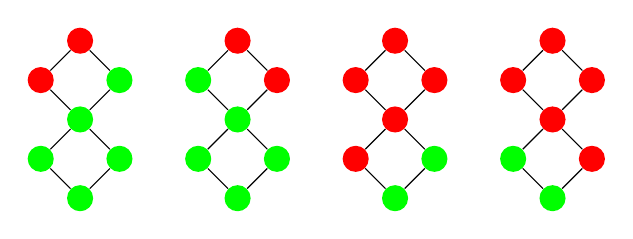
\begin{tikzpicture}[scale=0.5]
 \node (1) at (1,4) [circle,fill=red] {};
 \node (a) at (0,3) [circle,fill=red] {};
 \node (b) at (2,3) [circle,fill=green] {};
 \node (x) at (1,2) [circle,fill=green] {};
 \node (c) at (0,1) [circle,fill=green] {};
 \node (d) at (2,1) [circle,fill=green] {};
 \node (0) at (1,0) [circle,fill=green] {};
 \draw (1) edge (a) (1) edge (b);
 \draw (a) edge (x) (b) edge (x);
 \draw (x) edge (c) (x) edge (d);
 \draw (c) edge (0) (d) edge (0);

 \node (1s) at (5,4) [circle,fill=red] {};
 \node (as) at (4,3) [circle,fill=green] {};
 \node (bs) at (6,3) [circle,fill=red] {};
 \node (xs) at (5,2) [circle,fill=green] {};
 \node (cs) at (4,1) [circle,fill=green] {};
 \node (ds) at (6,1) [circle,fill=green] {};
 \node (0s) at (5,0) [circle,fill=green] {};
 \draw (1s) edge (as) (1s) edge (bs);
 \draw (as) edge (xs) (bs) edge (xs);
 \draw (xs) edge (cs) (xs) edge (ds);
 \draw (cs) edge (0s) (ds) edge (0s);

 \node (1ss) at (9,4) [circle,fill=red] {};
 \node (ass) at (8,3) [circle,fill=red] {};
 \node (bss) at (10,3) [circle,fill=red] {};
 \node (xss) at (9,2) [circle,fill=red] {};
 \node (css) at (8,1) [circle,fill=red] {};
 \node (dss) at (10,1) [circle,fill=green] {};
 \node (0ss) at (9,0) [circle,fill=green] {};
 \draw (1ss) edge (ass) (1ss) edge (bss);
 \draw (ass) edge (xss) (bss) edge (xss);
 \draw (xss) edge (css) (xss) edge (dss);
 \draw (css) edge (0ss) (dss) edge (0ss);

 \node (1sss) at (13,4) [circle,fill=red] {};
 \node (asss) at (12,3) [circle,fill=red] {};
 \node (bsss) at (14,3) [circle,fill=red] {};
 \node (xsss) at (13,2) [circle,fill=red] {};
 \node (csss) at (12,1) [circle,fill=green] {};
 \node (dsss) at (14,1) [circle,fill=red] {};
 \node (0sss) at (13,0) [circle,fill=green] {};
 \draw (1sss) edge (asss) (1sss) edge (bsss);
 \draw (asss) edge (xsss) (bsss) edge (xsss);
 \draw (xsss) edge (csss) (xsss) edge (dsss);
 \draw (csss) edge (0sss) (dsss) edge (0sss);
\end{tikzpicture} \]
\end{example}

A point in a topological space $X \in \mathbf{Top}$ is an element $x \in X$. This is equivalent to giving a monomorphism $* \xrightarrow{x} X$. This induces a surjective morphism of lattices $\mathcal{O}(X) \to \mathcal{O}(*) \cong [1]$.

\begin{theorem}
\label{boolean atoms are in bijection with maximal ideals}
Let $B$ be a complete boolean lattice. Then the set of atoms is in bijection with the set of maximal ideals.
\end{theorem}
\begin{proof}
Let $s \in B$ be an atom. 
Define $I[s] := \left\{ b \in B : b \wedge s = 0 \right\}$. 
Let $a,b \in I[s]$. 
Then $(a \vee b) \wedge s = (a \wedge s) \vee (b \wedge s) = 0 \vee 0 = 0$, hence $a \vee b \in I[s]$. 
If $a \in I[s]$ and $b \in B$ is such that $b \leq a$, then $b \wedge s = (b \wedge a) \wedge s = b \wedge (a \wedge s) = b \wedge 0 = 0$, hence $b \in I[s]$. 
So $I[s]$ is an ideal by \cref{prop:lattice ideals}. We will now show that $I[s]$ is prime (hence maximal). Assume that $a \wedge b \in I[s]$ and assume moreover that $a \not\in I[s]$. We want to show that $b \in I[s]$. Since $s$ is an atom, either $a \wedge s = 0$ or $a \wedge s = s$; thus $a \wedge s = s$. But $0 = (a \wedge b) \wedge s = b \wedge (a \wedge s) = b \wedge s$. Hence $b \in I[s]$. So $I[s]$ is prime.

Thus we found a function
\[ \varphi : \left\{\text{atoms of } B \right\} \to \Spec B, \qquad s \mapsto I[s]. \]
I claim that $\varphi$ is a bijection. Indeed if $s,t \in B$ are two distinct atoms ($s \neq t$), then $s \wedge t = 0$. Therefore $s \in I[t]$; but $s \not\in I[s]$. So $s \neq t \implies I[s] \neq I[t]$. To prove that $\varphi$ is surjective, we finally need completeness of $B$ (arbitrary joins). Consider the element
\[ s = \bigvee M = \bigvee_{m \in M} m \in B. \]
Note that $s \neq 1$; if it were then $M = B$. 
Hence $\neg s \neq 0$. I claim that $\neg s$ is an atom. 
So let $b \in B$ be an arbitrary element and consider $b \wedge \neg s$. 
If $b \in M$, then $\neg b \not\in M$ by \cref{boolean lattice prime is maximal}. 
So $\neg b \vee s = 1$. Hence $b \wedge \neg s = \neg (\neg b \vee s) = \neg 1 = 0$. 
If $b \not\in M$, then $\neg b \in M$ by \cref{boolean lattice prime is maximal}. 
So $\neg b \leq s$; thus $b \wedge \neg s = \neg s$. Hence $\neg s$ is an atom. Finally I claim that $\neg s$ is the atom we seek; i.e. I claim that $I[\neg s] = M$. It's easily checked that $a \in I[\neg s] \iff a \in M$, using that $\neg s$ is an atom and $s$ is the supremum over all elements of $M$.
\end{proof}

\begin{corollary}
\label{there exist boolean lattices with an empty spectrum}
There exist complete boolean lattices with an empty spectrum.
\end{corollary}
\begin{proof}
Take the free boolean lattice on a countably infinite set $\mathcal{B}S$. The boolean lattice $\mathcal{B}S$ has no atoms.
\end{proof}

\begin{corollary}
There exist toposes without points.
\end{corollary}
\begin{proof}
Let $B$ be a complete boolean lattice. Consider $B$ as a category in the usual way together with its canonical covering sieves $J$. 
Thus we have a Grothendieck topos $\Sh(B,J)$. Let $p : \mathbf{Sets} \to \Sh(B,J)$ be a point; i.e. a geometric morphism between toposes. 
We have an adjoint pair $p^* \dashv p_*$ such that $p^*$ is left-exact.
Now terminal objects and joins ($\vee$) are examples of colimits, so $p^*$ preserves them.
Binary meets $(\wedge)$ and monomorphisms are finite limits, so $p^*$ preserves them.
Hence $p^*$ sends subobjects to subobjects.
Subobjects of the terminal sheaf $1 \in \Sh(B,J)$ are representable subfunctors. 
So they are of the form $h_b$ with $b \in B$, where $h_b : B^{\op} \to \mathbf{Sets}$ is the Yoneda functor defined by $h_b(c) = \Hom(c,b)$.
The lattice formed by the subobjects of $1$ is precisely isomorphic to $B$ again. 
Hence we may restrict the functor $p^* : \Sh(B,J) \to \mathbf{Sets}$ to the boolean lattices $\Sub_{\Sh(B,J)}(1) \cong B \to \Sub_{\mathbf{Sets}}(1) \cong [1]$; in which case we may regard it as a homomorphism of bounded boolean lattices. But by \cref{prop:lattice ideals}, \cref{boolean lattice prime is maximal} and \cref{boolean atoms are in bijection with maximal ideals}, every such point $p$ of a topos gives us an atom. Hence if $B$ has no atoms, there are no points on the topos $\Sh(B,J)$. By \cref{there exist boolean lattices with an empty spectrum}, such boolean lattices exist.
\end{proof}

